\section{\Large{Introduction}}
% \begin{enumerate}[label=\arabic*]
%%%%%%%%%%%%%%%%%%%%%%%%%%%%%%%%%%%%%%%%%%%%
\subsection {\large{Motivation}} 
The IOT market has been growing rapidly in recent years. According to IOT Analytics, the IOT device market, which was valued at \$120 billion in 2019, is growing at a staggering rate, reaching \$100 billion in the first quarter of 2023. This market is also expected to grow at a CAGR of 20\% in the future. According to the same organization, there are currently an estimated 14.4 billion connected IOT devices, which is also expected to grow at a CAGR of 16\%. \\

\begin{figure}[ht]
    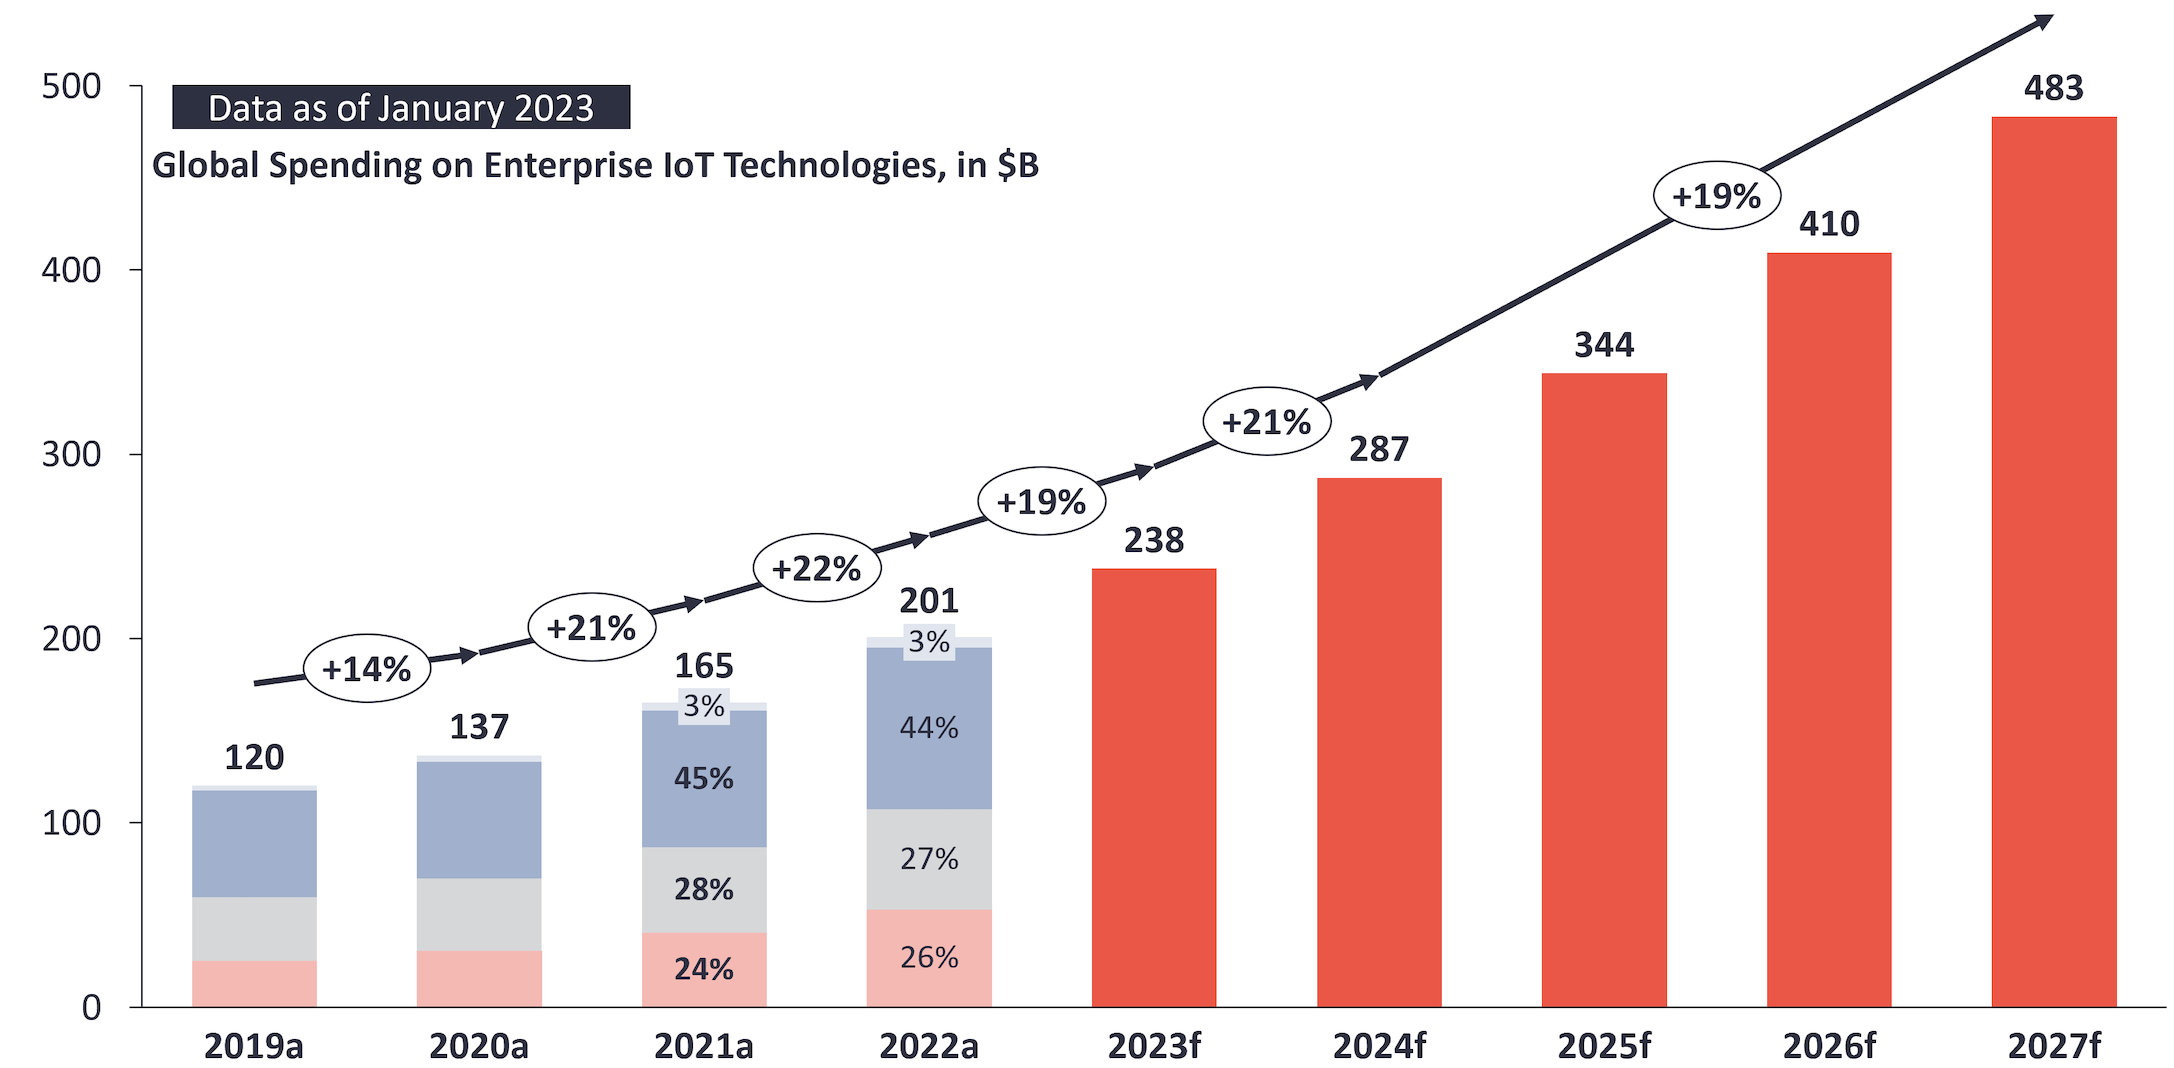
\includegraphics[width=8cm]{imgs/introduction/iot_market_growing.png}
    \caption{Growing IOT market}
    \renewcommand{\thefigure}{\thesubsection.\arabic{figure}}
\end{figure}

In response to this market growth, many electronics manufacturers have begun to include IOT-related technologies in their products, ranging from passive technologies that allow you to control your device through an application on your phone, to technologies that allow you to control multiple devices with a single device in conjunction with devices such as smart speakers, to more advanced technologies such as air quality sensors and motion recognition sensors that allow you to operate your device automatically without human command. \\

Consumer interest in IOT technologies is on the rise, and according to OpenSurvey, the number of consumers who own a home appliance with these technologies has grown from 29.5\% in 2022 to 48.3\% in 2023, an increase of 18.8 percentage points over the previous year.\cite{iot-market-size} \\\\

\begin{figure}[ht]
    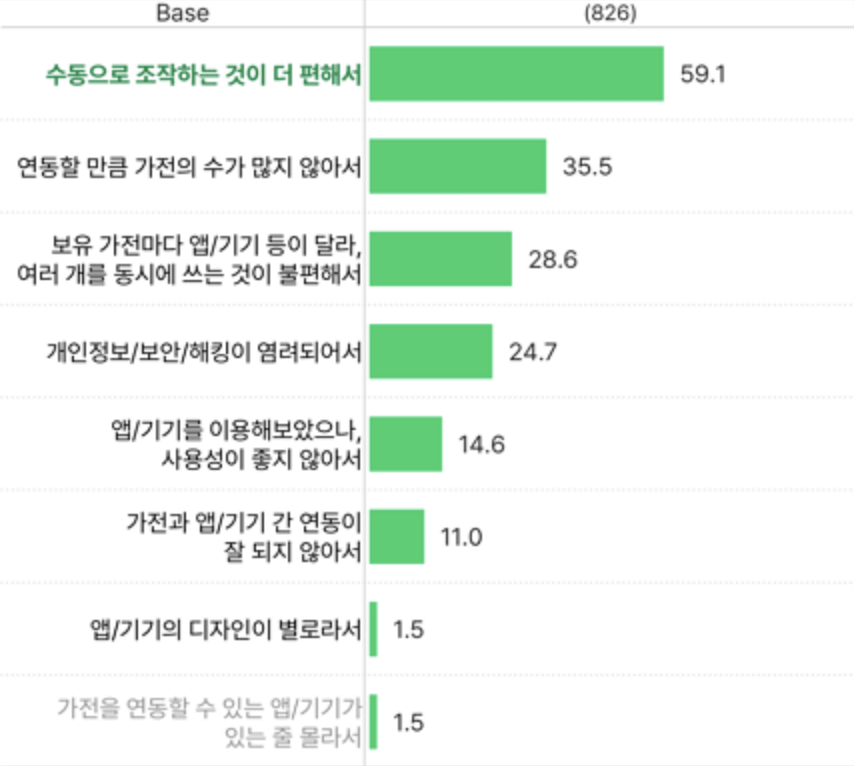
\includegraphics[width=8cm]{imgs/introduction/reason_why_not_use_iot.png}
    \caption{Reasons for not using IOT devices}
    \renewcommand{\thefigure}{\thesubsection.\arabic{figure}}
\end{figure}

However, consumers who have tried these technologies are often disappointed with devices that don't deliver on their pre-purchase expectations and stop using them. There are a few main reasons why this happens. According to OpenSurvey, these are the top reasons consumers have IOT devices but don't use them. \cite{iot-opensurvey}\\
\begin{enumerate}
    \item They are more comfortable operating them manually (59.1\%)\\
    \item They have different apps/devices for each device they own and don't want to use multiple devices at the same time (28.6\%)\\
    \item They have tried the apps/devices but don't like the usability (14.6\%)\\
    \item The apps/devices don't work well with their devices (11.0\%)\\
\end{enumerate}

We propose a platform to address the necessary issues for consumers to utilize IoT technologies. Our integrated IoT platform employs posture recognition to activate desired functions.\\\\

\newpage
%%%%%%%%%%%%%%%%%%%%%%%%%%%%%%%%%%%%%%%%%%%%
\subsection {\large{Problem Statement}}
    \begin{enumerate}[label=\alph*]
        \item Uncomfortable Automation\\
        There is a gap between what users think home automation should be and what current platforms offer. Users assume that machines will interpret their intentions and complete tasks without any input, but the reality is quite the opposite. The machines can only perform specific procedures that have already been entered, and they lack the ability to determine when those procedures should be executed. Currently, the sole means of inducing a machine to execute a task is through summoning a voice assistant with a designated command and directing it to execute a specific procedure. This hindrance fosters the belief that it is more convenient to manually operate a device than to avail oneself of automation. Consequently, users will avail themselves of IOT features only under highly restricted circumstances.\\
        
        \item Complexity of Use\\
        Currently, IOT devices from manufacturers and platforms can only be controlled through voice recognition. However, this method is too limited for users who desire a fully-fledged smart home. Third-party platforms exist for these users, which provide more detailed and advanced features. Although these platforms are not officially supported by the manufacturers, users who encounter problems must solve them on their own. Connecting devices to the platform and building the server are required tasks. Additionally, these platforms these platforms describe their behavior in code, which means users have to get used to it. These factors increase complexity and may present a barrier to entry for the users.\\
        
        \item Security Concerns\\
        Devices that use a manufacturer's platform can pose security risks by sending all user and device information to the manufacturer's servers. This compromise exposes sensitive personal information and lifestyle details to potential exploitation. Additionally, it opens up the possibility for malicious actors to manipulate and misuse devices in the home remotely.\\
        
        \item Disjointed communication methods\\
        Numerous communication methods are utilized in IoT devices these days, encompassing traditional WiFi and Bluetooth as well as UWB, RFID, Zigbee, Z-WAVE, XBee, LoRa, SigFox, and many others. Device manufacturers have selected one or more communication methods to construct their devices, resulting in consumers being limited to devices that use a specific communication method based on the hub they utilize.\\
        
        \begin{figure}[ht]
            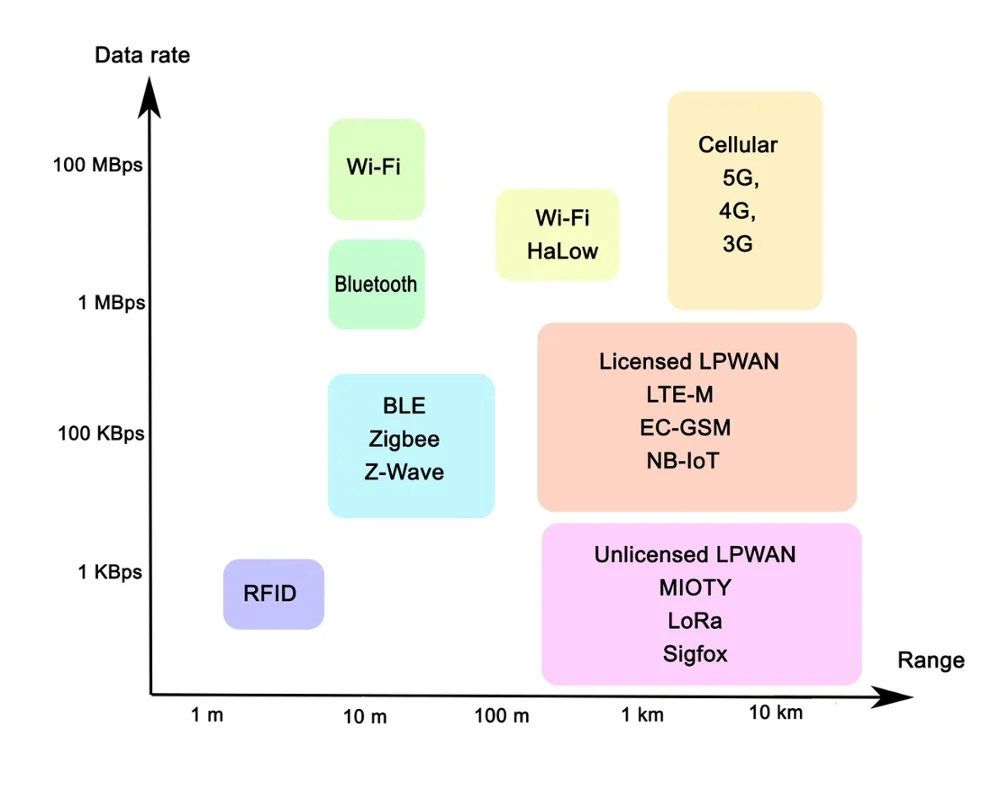
\includegraphics[width=7.5cm]{imgs/introduction/iot-protocols.png}
            \cite{iot-protocols}
            \caption{IOT protocols}
            \renewcommand{\thefigure}{\thesubsection.\arabic{figure}}
        \end{figure}
        
        \item Fragmented Platforms\\
        IOT device manufacturers maintain distinctive platforms and require navigating their platforms and hubs for using a specific device of a manufacturer. This limitation restricts the full functionality of devices to the manufacturer's designated platform, rendering interoperability difficult. Some manufacturer hubs do not allow devices from other manufacturers to connect, causing consumers to lean towards one manufacturer for their smart home devices and discouraging the use of products from different manufacturers at the same time. It also creates challenges when replacing a product line that is not made by a particular manufacturer, thus limiting consumer options.
        
    \end{enumerate}
%%%%%%%%%%%%%%%%%%%%%%%%%%%%%%%%%%%%%%%%%%%%
\subsection {\large{Related Software}}
    \begin{enumerate}[label=\alph*]
    \item Google Home\\
    This is a smart home platform offered by Google. It is compatible with a variety of devices, including lights, thermometers, speakers, and more. Additionally, it works with the Google Assistant, which allows you to check the status of your devices or control them. The same can be done through the accompanying application. Routines tailored to specific circumstances can be created and activated via voice commands. Easily add family members to share routines and jointly control devices. In addition to setting things up in the application, user can automate the details using YAML scripts.\\\\

    \item Apple Home\\
    This is a smart home platform offered by Apple that is compatible with a variety of devices including lights, thermometers, and speakers, among others. It works with the Siri, which allows you to check the status of your devices or control them. The same can be done through the accompanying application. One can conveniently monitor device status via Control Center or widgets on other Apple devices. An Apple TV can also serve as a hub and automatically regulate devices based on circumstance, including weather, motion, or humidity. However, an Apple device is required.\\\\

    \item Samsung Smartthings\\
    This is a smart home platform offered by Samsung. This platform is compatible with a variety of devices, including lights, thermometers, and speakers. Users can access and manage device status via Bixby or the application. To take full advantage of the IOT capabilities of their Samsung home appliances, users need this platform. User can utilize their Samsung devices as sensors. Unlike platforms offered by other manufacturers, Smartthings is an open platform, allowing for connection of even unsanctioned products through various actions. The hub permits connection of third-party sensors and setup of automation routines.\\\\

    \item LG ThinQ\\
    This is a smart home platform designed by LG that is necessary for full utilization of the IOT features of LG appliances. Users can receive notifications when their appliances finish their tasks, diagnose problems with their appliances, and schedule after-sales services. They can also integrate with Apple HomeKit to monitor or control their HomeKit-connected devices using this application.\\\\


    \item Home Assistant\\
    This is the sole mainstream smart home platform founded on open-source principles. The software can be installed and run on various hardware, including Raspberry Pi or Odroid. Devices with Home Assistant behave as hubs once the software is installed.\\
    
    \begin{figure}[ht]
        \begin{center}
            \raggedleft
            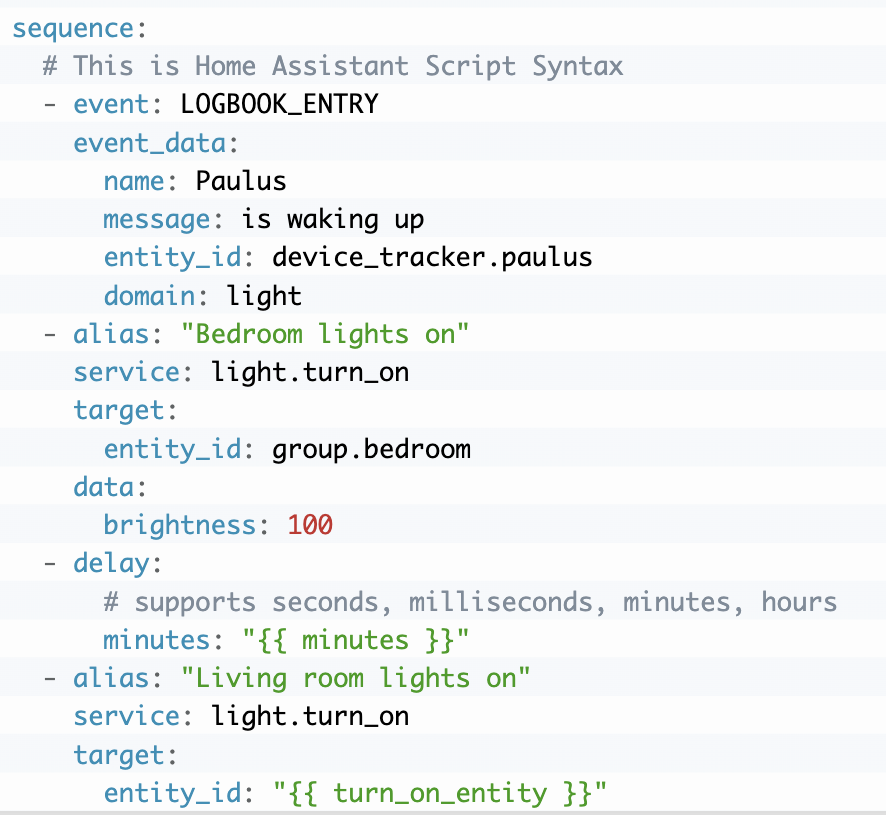
\includegraphics[width=8cm]{imgs/introduction/ha_script_example.png}
            \caption{Home Assistant script example}
            \renewcommand{\thefigure}{\thesubsection.\arabic{figure}}
        \end{center}
    \end{figure}
    
    It supports a diverse range of protocols and easily connects to devices unsupported by it through multiple actions. It is more difficult to configure than other platforms, but after mastering it, scripts can be utilized to access any data from linked devices and automate actions in numerous ways.\\
    

    \end{enumerate}